In previous sections, we have explained fundamental features of FDPS using relatively simple application codes. However, we need to develop a more complex application in actual research, in which for example we need to treat different types of particles. In this section, we will explain advanced features of FDPS using practical applications. \ul{To keep the explanations short and simple, we require the readers understand the contents of the previous sections in this document}.
%=============================
%   N-body+SPH code
%=============================
\subsection{$N$-body/SPH code} \label{subsec:NbodySPH}
In this section, we explain the accompanying sample code for $N$-body/SPH simulation of a disk galaxy. In this code, dark matter and stars, which perform gravitational interaction only, are represented by $N$-body particles, while interstellar gas, which performs both gravitational and hydrodynamic interactions, is represented by SPH particles. The tree method is used for the gravity calculation. The SPH scheme adopted in this code is the one proposed by \href{https://doi.org/10.1046/j.1365-8711.2002.05445.x}{Springel \& Hernquist [2002, MNRAS, 333, 649]} and \href{https://doi.org/10.1111/j.1365-2966.2005.09655.x}{Springel [2005, MNRAS, 364, 1105]} (hereafter, we call it Springel's SPH scheme). The readers can understand how to treat different types of particles using FDPS by reading this section.

Below, we first explain the usage of the code. Next, we give a brief explanation of the Springel's SPH scheme. Then, we explain the contents of the sample source codes in detail.

\subsubsection{How to run the sample code}
\label{subsubsec:NbodySPH_usage}
As we described, this code simulates the dynamical evolution of a disk galaxy. This code sets the initial distributions of dark matter and stars by reading a file created by \href{https://bitbucket.org/ymiki/magi}{\textsc{MAGI}} (\href{https://doi.org/10.1093/mnras/stx3327}{Miki \& Umemura [2018, MNRAS, 475, 2269]}), which is a software to make an initial condition of a galaxy simulation. On the other hand, the initial gas distribution is set inside the code. Therefore, the following procedures are required to use the code.
\begin{itemize}
\item Move to directory \dirNameNbodySPHSample
\item Edit \texttt{Makefile} in the current directory
\item Create particle data using \href{https://bitbucket.org/ymiki/magi}{\textsc{MAGI}} and place it under directory\texttt{./magi\_data/dat}
\item Run the \texttt{make} command to create the executable \texttt{nbodysph.out}
\item Run \texttt{nbodysph.out}
\item Check the output
\end{itemize}

Below, we explain each procedure.

\subsubsubsection{Move to the directory the sample code is placed}
\label{s3sec:NbosySPH_code_loc}
Move to \dirNameNbodySPHSample.

\subsubsubsection{File structure of the sample code}
\label{s3sec:NbodySPH_file_str}
The following is the file structure of the sample code.
\ifCpp % for C++
\begin{screen}
\begin{verbatim}
$ ls | awk '{print $0}'
Makefile
Makefile.K
Makefile.ofp
ic.hpp
job.K.sh
job.ofp.sh
leapfrog.hpp
macro_defs.hpp
magi_data/
main.cpp
mathematical_constants.cpp
mathematical_constants.h
physical_constants.cpp
physical_constants.h
test.py*
user_defined.hpp
\end{verbatim}
\end{screen}
We explain briefly the content of each source file. In \texttt{ic.hpp}, functions to create initial conditions are implemented. Users can choose an initial condition other than that for a disk galaxy (described later). In \texttt{leapfrog.hpp}, we implement functions necessary to integrate the orbits of particles based on the Leapfrog method. In \texttt{macro\_defs.hpp}, we define macros that are used to control numerical simulation. In \texttt{main.cpp}, the main routine is implemented. In \texttt{mathematical\_constants.h} and \texttt{mathematical\_constants.cpp}, we define some mathematical constants. In \texttt{physical\_constants.h} and \texttt{physical\_constants.cpp}, we define some physical constants. In \texttt{user\_defined.hpp}, we define user-defined classes and interaction functions.
\endifCpp
\ifFtn % for Fortran
\begin{screen}
\begin{verbatim}
$ ls | awk '{print $0}'
Makefile
Makefile.K
Makefile.intel
Makefile.ofp
f_main.F90
ic.F90
job.K.sh
job.ofp.sh
leapfrog.F90
macro_defs.h
magi_data/
mathematical_constants.F90
physical_constants.F90
test.py
tipsy_file_reader.cpp
tipsy_file_reader.h
user_defined.F90
\end{verbatim}
\end{screen}
We explain briefly the content of each source file. In \texttt{ic.F90}, subroutines to create initial conditions are implemented. Users can choose an initial condition other than that for a disk galaxy (described later). In \texttt{leapfrog.F90}, we implement subroutines necessary to integrate the orbits of particles based on the Leapfrog method. In \texttt{macro\_defs.h}, we define macros that are used to control numerical simulation. In \texttt{f\_main.F90}, the main routine is implemented. In \texttt{mathematical\_constants.F90}, we define some mathematical constants. In \texttt{physical\_constants.F90}, we define some physical constants. In \texttt{tipsy\_file\_reader.*}, we define functions to read particle data created by \textsc{MAGI}. In \texttt{user\_defined.F90}, we define user-defined types and interaction functions.
\endifFtn
\ifC % for C
\begin{screen}
\begin{verbatim}
$ ls | awk '{print $0}'
Makefile
Makefile.ofp
c_main.c
ic.c
ic.h
job.ofp.sh
leapfrog.c
leapfrog.h
macro_defs.h
magi_data/
mathematical_constants.c
mathematical_constants.h
physical_constants.c
physical_constants.h
tipsy_file_reader.cpp
tipsy_file_reader.h
user_defined.c
user_defined.h
\end{verbatim}
\end{screen}
We explain briefly the content of each source file. In \texttt{ic.*}, functions to create initial conditions are implemented. Users can choose an initial condition other than that for a disk galaxy (described later). In \texttt{leapfrog.*}, we implement functions necessary to integrate the orbits of particles based on the Leapfrog method. In \texttt{macro\_defs.h}, we define macros that are used to control numerical simulation. In \texttt{c\_main.c}, the main function is implemented. In \texttt{mathematical\_constants.*}, we define some mathematical constants. In \texttt{physical\_constants.*}, we define some physical constants. In \texttt{tipsy\_file\_reader.+}, we define functions to read particle data created by \textsc{MAGI}. In \texttt{user\_defined.*}, we define user-defined types and interaction functions.
\endifC

Directory \texttt{magi\_data} stores a parameter file input to the software \textsc{MAGI} (\texttt{magi\_data/cfg/*}) and a script file used to run \textsc{MAGI} (\texttt{magi\_data/sh/run.sh}).

\subsubsubsection{Edit Makefile}
\label{s3sec:NbodySPH_Makefile}
Edit \path{Makefile} following the description below.
\begin{itemize}
\item Set the variable \path{CXX} the command to run your C++ compiler.
\ifFtn % for Fortran
\item Set the variable \path{FC} the command to run your Fortran compiler.
\endifFtn
\ifC % for C
\item Set the variable \path{CC} the command to run your C compiler.
\endifC
\item Set the variable \path{CXXFLAGS} compile options of the C++ compiler.
\ifFtn % for Fortran
\item Set the variable \path{FCFLAGS} compile options of the Fortran compiler.
\endifFtn
\ifC % for C
\item Set the variable \path{CFLAGS} compile options of the C compiler.
\endifC
\item In this code, several macros are used to control numerical simulations. Table \ref{tbl:NbodySPH:compile_time_macros} lists the names of the macros and their definitions. In addition, there are macros whose states (i.e. value or defined/undefined states) are automatically set according to the value of macro \path{INITIAL_CONDITION}. Generally, users do not have to change them. Please see \path{macro_defs.h} directly for detail.
\item Phantom-GRAPE library for x86 can be used for the gravity calculation. To use it, set the variable \path{use_phantom_grape_x86} \path{yes}.
\end{itemize}
As for the way to specify the use/non-use of OpenMP and MPI, see \S~\ref{sec:getting_started}.


\begin{table}[H]
\begin{tabularx}{\linewidth}{|c|X|}
\toprule
\rowcolor{Snow2}
Macro name & Defintion \\
\midrule
\path{INITIAL_CONDITION} & It specifies the type of initial condition or the operation mode of the code. It must take a value from 0 to 3. According to its value, the code operates as follows. 0: an initial condition for a disk galaxy is used, 1: an initial condition for cold collapse test problem is used, 2: an initial condition for Evrard test is used, 3: the code operates in the mode to make a glass-like distribution of SPH particles. \\
\midrule
\path{ENABLE_VARIABLE_SMOOTHING_LENGTH} & It specifies that smoothing length of SPH particles is variable or not. If it is defined, variable smoothing length is used and the SPH calculation is performed according to the Springel's SPH scheme. If it is not defined, the fixed smoothing length is used and the SPH calculation is done in almost the same way as the sample code described in \S~\ref{sec:getting_started}-\ref{sec:how_to_use}. \\
\midrule
\path{USE_ENTROPY} & It specifies whether to use entropy or specific internal energy as an independent variable to describe the thermodynamic state of SPH particle. If defined, entropy is used. But, if macro \path{ISOTHERMAL_EOS} described below is defined, specific internal energy is forcibly used (specific internal energy is used to calculate pressure). \\
\midrule
\path{USE_BALSARA_SWITCH} & It specifies whether Balsara switch (\href{https://doi.org/10.1016/S0021-9991(95)90221-X}{Balsara [1995, JCP, 121, 357]}) is used or not. If defined, the Balsara switch is used. \\ 
\midrule
\path{USE_PRESCR_OF_THOMAS_COUCHMAN_1992} & It specifies whether a simple prescription proposed by \href{https://doi.org/10.1093/mnras/257.1.11}{Thomas \& Couchman [1992, MNRAS,257, 11]} to prevent the tensile instability is used or not. If defined, this prescription is used. \\
\midrule
\path{ISOTHERMAL_EOS} & It specifies whether isothermal process is assumed or not. If defined, isothermal process is assumed (specific internal energy is assumed to be constant). If not defined, the code solve the entropy equation or the internal energy equation.\\
\midrule
\path{READ_DATA_WITH_BYTESWAP} & It specifies whether the program reads particle data with performing byte swap (byte swap is applied for each variable of basic data type). If defined, byte swap is performed.\\
\bottomrule
\end{tabularx}
\caption{Compile-time macros and their definitions}
\label{tbl:NbodySPH:compile_time_macros}
\end{table}

\subsubsubsection{Create particle data using MAGI}
\label{s3sec:NbodySPH_MAGI_usage}
As described earlier, users need to create particle data using the software \textsc{MAGI} before simulation according to the procedures described below. For users who cannot use \texttt{MAGI} for some reasons, we prepared sample particle data in web sites described below. In the following, we explain each case in detail.
\begin{description}
\item[Create particle data using \textsc{MAGI}] Create particle data as follows.
\begin{enumerate}
\item Download the source file of \textsc{MAGI} from the web side \href{https://bitbucket.org/ymiki/magi}{https://bitbucket.org{\slash}ymiki{\slash}magi} and install it in appropriate PATH according to the descriptions in Section ``How to compile MAGI" in the above web side. \ul{But, our {$N$}-body/SPH sample code supports TIPSY file format only. Therefore, please build {\textsc{MAGI}} with {\path{USE_TIPSY_FORMAT=ON}}}.
\item Edit \texttt{./magi\_data/sh/run.sh} and set the variable \path{MAGI_INSTALL_DIR} the PATH of the directory where the \texttt{magi} command is stored. Also, set the variable \texttt{NTOT} the number of $N$-body particles (\textsc{MAGI} automatically assigns the numbers of dark matter particles and star particles).
\item Edit \texttt{./magi\_data/cfg/*} to specify a galaxy model. For detail of the format of input file for \textsc{MAGI}, please see the web side above or Section 2.4 in the original paper \href{https://doi.org/10.1093/mnras/stx3327}{Miki \& Umemura [2018, MNRAS, 475, 2269]}. In the default, galaxy model consists of the following four components (hereafter, we call this \textbf{default galaxy model}):
\begin{enumerate}[label=(\roman*)]
\item Dark matter halo (NFW profile, $M=10^{12}\;\mathrm{M_{\odot}}$, $r_{s}=21.5\;\mathrm{kpc}$, $r_{c}=200\;\mathrm{kpc}$, $\Delta_{c}=10\;\mathrm{kpc}$)
\item Stellar bulge (King model, $M=5\times 10^{10}\;\mathrm{M_{\odot}}$, $r_{s}=0.7\;\mathrm{kpc}$, $W_{0}=5$)
\item Thick stellar disk  (S{\'e}rsic profile, $M=2.5\times 10^{10}\;\mathrm{M_{\odot}}$, $r_{s}=3.5\;\mathrm{kpc}$, $n=1.5$, $z_{d}=1\;\mathrm{kpc}$, $Q_{T,\min}=1.0$)
\item Thin stellar disk (exponential disk, $M=2.5\times 10^{10}\;\mathrm{M_{\odot}}$, $r_{s}=3.5\;\mathrm{kpc}$, $z_{d}=0.5\;\mathrm{kpc}$, $Q_{T,\min}=1.0$)
\end{enumerate}
In the default galaxy model, two stellar disks are marginally unstable to a bar-mode in view of the Ostriker-Peebles criterion. Therefore, a simulated galaxy is expected to evolve into a spiral galaxy having a weak bar. In the latest release of \textsc{MAGI} (version 1.1.1 [as of July 19th, 2019]), its default operation mode is changed from previous releases. With this demand, we have replaced parameter $f$ in thick and thin disks by $Q_{T,\min}$, where $f$ is a parameter controlling the velocity dispersion of disk and is used in the previous releases of \textsc{MAGI} to specify the stability of a disk component. $Q_{T,\min}$ is the minimum of Toomre Q value in the disk. (In the sample code in FDPS 5.0d or earlier, we used $f=0.125$).
\item Move to directory \texttt{magi\_data} and run the following command:
\begin{screen}
\$ ./sh/run.sh
\end{screen}
\item If \textsc{MAGI} stops successfully, particle data whose extension is \texttt{tipsy} will be created in directory \path{magi_data/dat}.
\end{enumerate}
\item[Download sample particle data form our web sites]  Download a particle data file from one of the following URLs and place it under directory \texttt{./magi\_data/dat/}. All of particle data is made with the default galaxy model. Only the number of particles is different for each data.
\begin{itemize}
\item $N=2^{21}$: \url{https://v2.jmlab.jp/owncloud/index.php/s/XnzvW5XAYwfqZYQ/download?path=%2Fmagi_data%2FGalaxy%2F21&files=Galaxy.tipsy}
\item $N=2^{22}$: \url{https://v2.jmlab.jp/owncloud/index.php/s/XnzvW5XAYwfqZYQ/download?path=%2Fmagi_data%2FGalaxy%2F22&files=Galaxy.tipsy}
\item $N=2^{23}$: \url{https://v2.jmlab.jp/owncloud/index.php/s/XnzvW5XAYwfqZYQ/download?path=%2Fmagi_data%2FGalaxy%2F23&files=Galaxy.tipsy}
\item $N=2^{24}$: \url{https://v2.jmlab.jp/owncloud/index.php/s/XnzvW5XAYwfqZYQ/download?path=%2Fmagi_data%2FGalaxy%2F24&files=Galaxy.tipsy}
\end{itemize}
\end{description}

\subsubsubsection{Run make}
\label{s3sec:NbodySPH_make}
Type ``make'' to run the \path{make} command.

\subsubsubsection{Run the sample code}
\label{s3sec:NbodySPH_execution}
\begin{itemize}
\item If you are not using MPI, run the following in CLI (terminal)
\begin{screen}
\begin{verbatim}
$ ./nbodysph.out
\end{verbatim}
\end{screen}
  
\item If you are using MPI, run the following in CLI (terminal)
\begin{screen}
\begin{verbatim}
$ MPIRUN -np NPROC ./nbodysph.out
\end{verbatim}
\end{screen}
where \texttt{MPIRUN} should be \texttt{mpirun} or \texttt{mpiexec} depending on your MPI configuration, and \texttt{NPROC} is the number of processes you will use.
\end{itemize}

\subsubsubsection{Analysis of the result}
\label{s3sec:NbodySPH_result_analysis}
\ifCpp % for C++
In the directory \path{result}, data of $N$-body and SPH particles are output as files ``nbody0000x.dat" and ``sph0000x.dat", where x is an integer representing time.
\endifCpp
\ifIF % for Fortran and C
In the directory \path{result}, data of $N$-body and SPH particles are output as files ``nbody0000x-proc0000y.dat" and ``sph0000x-proc0000y.dat", where x is an integer representing time and y is an integer representing a process number (MPI rank number).
\endifIF
The output file format of $N$-body particle data is that in each line, index of particle, mass, position (x, y, z), velocity (vx, vy, vz) are listed. The output file format of SPH particle data is that in each line, index of particle, mass, positon (x, y, z), velocity (vx, vy, vz), density, specific internal energy, entropy, pressure are listed.

Figure~\ref{fig:nbodysph} shows the distribution of star and SPH particles at $T=0.46$ for a disk galaxy simulation with the number of $N$-body particles is $2^{21}$ and the number of SPH particles is $2^{18}$.

\begin{figure}[h]
\centering
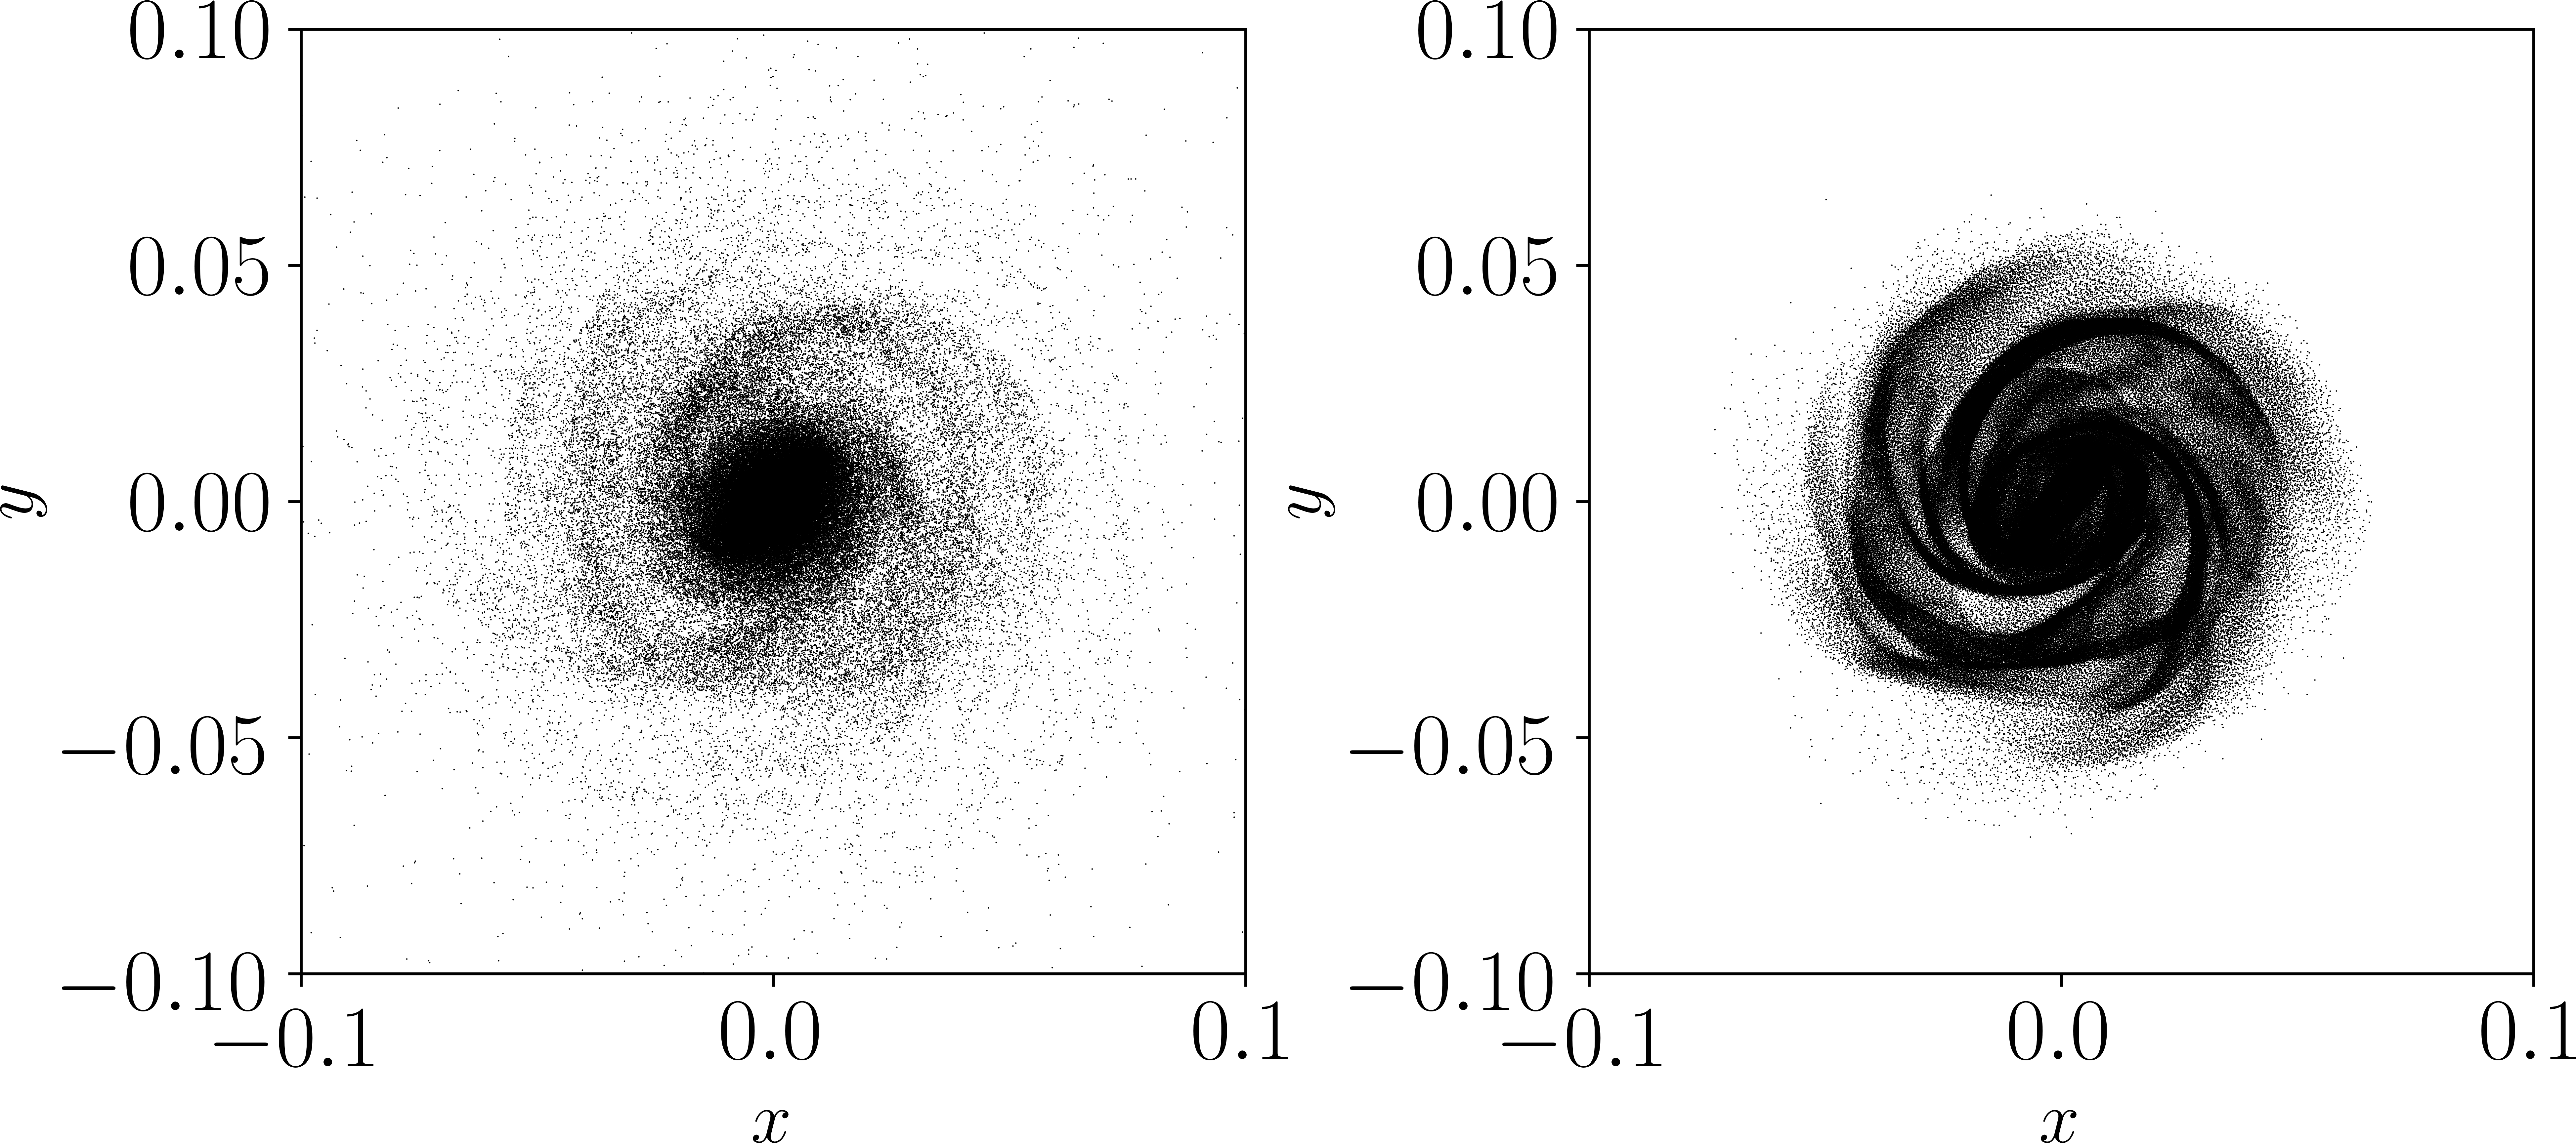
\includegraphics[width=\linewidth]{./fig/nbodysph_t046.png}
\caption{Face-on view of distributions of stars (left) and gas (right) (simulation configuration: the simulation is performed the number of $N$-body particles is $2^{21}$, the number of SPH particles is $2^{18}$, isothermal, gas temperature is $10^{4}\;\mathrm{K}$, mean molecular weight to the mass of hydrogen $\mu=0.5$)}
\label{fig:nbodysph}
\end{figure}


Below, we briefly explain the Springel's SPH scheme and then explain the implementation of the sample code.


\subsubsection{Springel's SPH scheme}
\label{subsubsec:Springel_scheme}
\href{https://doi.org/10.1046/j.1365-8711.2002.05445.x}{Springel \& Hernquist [2002, MNRAS, 333, 649]} proposed a formulation of SPH (actually, equation of motion[EoM]) where the total energy and entropy of a system are conserved even if smoothing length changes with time. In this section, we briefly explain their formulation. The outline of the derivation is as follows. Construct a Lagrangian of the system assuming that smoothing length is also independent variable, then solve the Euler-Lagrange equations under $N$ constraints, where $N$ is the number of particles.

More specifically, they consider the Lagrangian
\begin{equation}
L(\bm{q}, \dot{\bm{q}}) = \dfrac{1}{2}\sum^{N}_{i=1}m_{i}\dot{\bm{r}}^{2}_{i} - \dfrac{1}{\gamma -1}\sum^{N}_{i=1}m_{i}A_{i}\rho^{\gamma-1}_{i} \label{eq:Lagrangian}
\end{equation}
where $\bm{q}=(\bm{r}_{1},...,\bm{r}_{N},h_{1},...h_{N})$ is the generalized coordinates (the subscripts represent the indice of particles), $\bm{r}_{i}$ is the position, $h_{i}$ is smoothing length, $m_{i}$ is mass, $\gamma$ is the ratio of specific heats, $\rho_{i}$ is density, $A_{i}$ is called entropy function and it is related with specific internal energy $u_{i}$ and $\rho_{i}$ through the equation
\begin{equation}
u_{i} = \dfrac{A_{i}}{\gamma-1}\rho^{\gamma-1}_{i} \label{eq:relation_between_u_A_rho}
\end{equation}
The first and second terms of Eq.(\ref{eq:Lagrangian}) represents the kinetic energy and the internal energy of the system, respectively. Because solving the Euler-Lagrangian equation directly using this Lagrangian results in $4N$ equations, which is not undesirable, they introduce the following $N$ constraints.
\begin{equation}
\phi_{i} = \dfrac{4\pi}{3}h^{3}_{i}\rho_{i} - \overline{m}N_{\mathrm{neigh}}=0 \label{eq:Springel_SPH_constraints}
\end{equation}
where $\overline{m}$ is the average mass of SPH particles\footnote{This must be treated as constant.}, $N_{\mathrm{neigh}}$ is the number of neighbor particles (constant). Under these constraints, using the method of Lagrange multiplier, they solve the Euler-Lagrange equations to obtain the following equations of motion:
\begin{equation}
\dfrac{\mathrm{d}\bm{v}_{i}}{\mathrm{d}t} = - \sum^{N}_{j=1}m_{j}\left[f_{i}\dfrac{P_{i}}{\rho^{2}_{i}}\nabla_{i}W(r_{ij},h_{i})+f_{j}\dfrac{P_{j}}{\rho^{2}_{j}}\nabla_{i}W(r_{ij},h_{j})\right] \label{eq:Springel_SPH_EoM_pure_hydro}
\end{equation}
where $P_{i}$ is pressure, $r_{ij}=|\bm{r}_{i}-\bm{r}_{j}|$, $W$ is the kernel function, $f_{i}$ is the so-called $\nabla h$ term, defined by
\begin{equation}
f_{i} = \left(1 + \dfrac{h_{i}}{3\rho_{i}}\dfrac{\partial \rho_{i}}{\partial h_{i}}\right)^{-1} \label{eq:gradh_term}
\end{equation}

The thermodynamic state of the system is described by the independent variable $A_{i}$, the entropy. If the flow is adiabatic, the entropy is constant along the flow except for locations of shock waves where the entropy is increased. \href{https://doi.org/10.1111/j.1365-2966.2005.09655.x}{Springel [2005, MNRAS, 364, 1105]} modeled the increase of the entropy by passing shock waves using the method of artificial viscosity:
\begin{align}
\dfrac{\mathrm{d}A_{i}}{\mathrm{d}t} & = \dfrac{1}{2}\dfrac{\gamma-1}{\rho^{\gamma-1}_{i}}\sum^{N}_{j=1}m_{j}\Pi_{ij}\bm{v}_{ij}\cdot\nabla_{i}\overline{W}_{ij} \label{eq:Springel_SPH_entropy_eq} \\
\left.\dfrac{\mathrm{d}\bm{v}_{i}}{\mathrm{d}t}\right|_{\mathrm{visc}} & = -\sum^{N}_{j=1}m_{j}\Pi_{ij}\nabla_{i}\overline{W}_{ij} \label{eq:Springel_SPH_EoM_art_vis}
\end{align}
where $\bm{v}_{ij}=\bm{v}_{i}-\bm{v}_{j}$, $\bm{v}_{i}$ is velocity, $\overline{W}_{ij}=\frac{1}{2}(W(r_{ij},h_{i})+W(r_{ij},h_{j}))$. For $\Pi_{ij}$, please see the original papers.

The procedures of SPH calculation is summarized as follows:
\begin{screen}
\begin{enumerate}[leftmargin=*,itemsep=-1ex,label={(\arabic*)}]
\item Solve Eq.(\ref{eq:Springel_SPH_constraints}) and the following equation self-consistently to determine the density $\rho_{i}$ and the smoothing length $h_{i}$.
\begin{equation}
\rho_{i} = \sum^{N}_{j=1}m_{j}W(r_{ij},h_{i}) \label{eq:SPH_density_def}
\end{equation}
\item Calculate $\nabla h$ term defined by Eq.(\ref{eq:gradh_term}).
\item Calculate the right-hand side of Eqs.(\ref{eq:Springel_SPH_EoM_pure_hydro}), (\ref{eq:Springel_SPH_entropy_eq})、(\ref{eq:Springel_SPH_EoM_art_vis}).
\item Update the positions, velocities, entropies of SPH particles.
\end{enumerate}
\end{screen}


In the remaining sections, we first explain the implementations of user-defined classes and interaction functions. Then, we explain the implementation of the main routine where we explain how to treat different types of particles in FDPS.

\subsubsection{User-defined types}
All user-defined types are defined in \describeForEach{\path{user_defined.hpp}}{\path{user_defined.F90}}{\path{user_defined.h}}. Here, we explain the types of user-defined types used in this code. As described earlier, this code use two types of particles, $N$-body and SPH particles. Thus, this code defines \textbf{two} \textsf{FullParticle} types (\describeForEach{\texttt{FP\_nbody} class}{\texttt{fp\_nbody} type}{\texttt{fp\_nbody} type} for $N$-body particles and \describeForEach{\texttt{FP\_sph} class}{\texttt{fp\_sph} type}{\texttt{fp\_sph} type} for SPH particles). The number of types of \textit{physical} interactions are two, the gravitational and hydrodynamic interactions. But, as explained in \S~\ref{sec:how_to_use}, we need to perform (at least) two interaction calculations (for density and acceleration) in SPH calculations. Therefore, the code defines \textbf{three} \textsf{Force} types (\describeForEach{\texttt{Force\_grav} class}{\texttt{force\_grav} type}{\texttt{force\_grav} type} for the gravity calculation, \describeForEach{\texttt{Force\_dens} class}{\texttt{force\_dens} type}{\texttt{force\_dens} type} for the density calculation, and \describeForEach{\texttt{Force\_hydro} class}{\texttt{force\_hydro} type}{\texttt{force\_hydro} type} for the calculation of acceleration due to pressure gradient (hereafter we call it pressure-gradient acceleration for simplicity)). For simplicity, this code uses one \structure for both \textsf{EssentialParticleI} type and \textsf{EssentialParticleJ} type (hereafter, we call them together \textsf{EssentialParticle} type). Also this code uses the same \textsf{EssentialParticle} type for the calculations of density and pressure-gradient acceleration. Therefore, the number of types of \textsf{EssentialParticle} types is \textbf{two} (\describeForEach{\texttt{EP\_grav} class}{\texttt{ep\_grav} type}{\texttt{ep\_grav} type} for the gravity calculation and \describeForEach{\texttt{EP\_hydro} class}{\texttt{ep\_hydro} type}{\texttt{ep\_hydro} type} for SPH calculation).

Below, we explain the implementation of each user defined type.

%------------------------
%   FullParticle type
%------------------------
\subsubsubsection{FullParticle type}
First, we explain \describeForEach{\texttt{FP\_nbody} class}{\structure \texttt{fp\_nbody}}{\structure \texttt{fp\_nbody}}, which is used to store the information of $N$-body particles. This data type contains all physical quantities that a $N$-body particle should have as member variables. Listing \ref{nbodysph_FP_nbody} shows the implementation of \describeForEach{\texttt{FP\_nbody} class}{\texttt{fp\_nbody} type}{\texttt{fp\_nbody} type}. The definitions of the member variables \describeForCpp{and member functions} are almost the same as those of $N$-body sample code introduced in \S~\ref{sec:getting_started}-\ref{sec:how_to_use}. Thus, please see the corresponding section for detail.

\ifCpp % for C++
\lstinputlisting[linerange={146-180},caption=\textsf{FullParticle} type (\texttt{FP\_nbody} class),label=nbodysph_FP_nbody]{../../../../sample/c++/nbody+sph/user_defined.hpp}
\endifCpp
\ifFtn % for Fortran
\lstinputlisting[linerange={47-56},caption=\textsf{FullParticle} type (\texttt{fp\_nbody} type),label=nbodysph_FP_nbody]{../../../../sample/fortran/nbody+sph/user_defined.F90}
\endifFtn
\ifC % for C
\lstinputlisting[linerange={40-48},caption=\textsf{FullParticle} type (\texttt{fp\_nbody} type),label=nbodysph_FP_nbody]{../../../../sample/c/nbody+sph/user_defined.h}
\endifC


Next, we explain \describeForEach{\texttt{FP\_sph} class}{\structure \texttt{fp\_sph}}{\structure \texttt{fp\_sph}}, which is used to store the information of SPH particles. This data type contains all physical quantities that a SPH particle should have as member variables. Listing \ref{nbodysph_FP_sph} shows the implementation of \describeForEach{\texttt{FP\_sph} class}{\texttt{fp\_sph} type}{\texttt{fp\_sph} type}. The definitions of main member variables are as follows: \texttt{id} (identification number), \texttt{mass} (mass), \texttt{pos} (position[$\bm{r}_{i}$]), \texttt{vel} (velocity[$\bm{v}_{i}$]), \texttt{acc\_grav} (gravitational acceleration), \texttt{pot\_grav} (gravitational potential), \texttt{acc\_hydro} (pressure-gradient acceleration), \texttt{dens} (density[$\rho_{i}$]), \texttt{eng} (specific internel energy[$u_{i}$]), \texttt{ent} (entropy function [hereafter, entropy][$A_{i}$]), \texttt{pres} (pressure[$P_{i}$]), \texttt{smth} (smoothing length\footnote{It is defined as the distance from the center of a particle where the value of the SPH kernel function is 0.}[$h_{i}$]), \texttt{gradh} ($\nabla h$ term[$f_{i}$]), \texttt{divv} ($(\nabla\cdot\bm{v})_{i}$, where the subscript $i$ means that the derivative is performed at particle position), \texttt{rotv} ($(\nabla\times\bm{v})_{i}$), \describeForEach{\texttt{BalSW}}{\texttt{balsw}}{\texttt{balsw}} (coefficient for Balsara switch and its definition is the same as $f(a)$ in \href{https://doi.org/10.1016/S0021-9991(95)90221-X}{Balsara [1995, JCP, 121, 357]}), \texttt{snds} (sound speed), \texttt{eng\_dot} (time rate of change of \texttt{eng}), \texttt{ent\_dot} (time rate of change of \texttt{ent}), \texttt{dt} (the maximum allowable time step to integrate the orbit of this particle).

\ifCpp % for C++
The configuration of member functions are almost the same as those of the SPH sample code introduced in \S~\ref{sec:getting_started}-\ref{sec:how_to_use}, but there are the following differences:
\begin{itemize}[leftmargin=*,itemsep=-1ex]
\item SPH particles are involved with three types of interaction calculations (gravity, density, pressure-gradient acceleration). Thus, \textbf{three} types of member function \texttt{copyFromForce} are defined.
\item The existence of member function \texttt{writeBinaryPos}. This function is only used in the case of \path{INITIAL_CONDITION=3}.
\item The existence of member function \texttt{setEntropy}. This function is used to set the initial value of entropy.
\end{itemize}
For the other member functions, please see \S~\ref{sec:getting_started}-\ref{sec:how_to_use}.
\endifCpp 
\ifIF % for Fortran and C
The following points should be noted.
\begin{itemize}[leftmargin=*,itemsep=-1ex]
\item SPH particles are involved with three types of interaction calculations (gravity, density, pressure-gradient acceleration). Thus, \textbf{three} types of \texttt{copyFromForce} directives are written.
\end{itemize}
\endifIF

\ifCpp % for C++
\lstinputlisting[linerange={182-285},caption=\textsf{FullParticle} type (\texttt{FP\_sph} class),label=nbodysph_FP_sph]{../../../../sample/c++/nbody+sph/user_defined.hpp}
\endifCpp
\ifFtn % for Fortran
\lstinputlisting[linerange={58-86},caption=\textsf{FullParticle} type (\texttt{fp\_sph} type),label=nbodysph_FP_sph]{../../../../sample/fortran/nbody+sph/user_defined.F90}
\endifFtn
\ifC % for C
\lstinputlisting[linerange={50-78},caption=\textsf{FullParticle} type (\texttt{fp\_sph} type),label=nbodysph_FP_sph]{../../../../sample/c/nbody+sph/user_defined.h}
\endifC

%----------------------------
%   EssentialParticle type
%----------------------------
\subsubsubsection{EssentialParticle type}
First, we explain \describeForEach{\texttt{EP\_grav} class}{\structure \texttt{ep\_grav}}{\structure \texttt{ep\_grav}}, which is used for the gravity calculation. This data type has all physical quantities that $i$- and $j$-particles should have in order to perform gravity calculation as member variables. Listing \ref{nbodysph_EP_grav} shows the implementation of \describeForEach{\texttt{EP\_grav} class}{\texttt{ep\_grav} type}{\texttt{ep\_grav} type}. 
\ifCpp % for C++
\textsf{EssentialParticle} type should have member function(s) \texttt{copyFromFP()} to copy data from a \textsf{FullParticle} type. In this code, there are two \textsf{FullParticle} types and hence \textbf{two} \texttt{copyFromFP} functions are defined.
\endifCpp
\ifIF % for Fortran and C
\textsf{EssentialParticle} type should have \texttt{copyFromFP} directive(s) to specify the way of copy data from \textsf{FullParticle} type(s). In this code, there are two \textsf{FullParticle} types and hence \textbf{two} \texttt{copyFromFP} directives are written.
\endifIF

\ifCpp % for C++
\lstinputlisting[linerange={288-310},caption=\textsf{EssentialParticle} type (\texttt{EP\_grav} class),label=nbodysph_EP_grav]{../../../../sample/c++/nbody+sph/user_defined.hpp}
\endifCpp
\ifFtn % for Fortran
\lstinputlisting[linerange={89-95},caption=\textsf{EssentialParticle} type (\texttt{ep\_grav} type),label=nbodysph_EP_grav]{../../../../sample/fortran/nbody+sph/user_defined.F90}
\endifFtn
\ifC % for C
\lstinputlisting[linerange={81-87},caption=\textsf{EssentialParticle} type (\texttt{ep\_grav} type),label=nbodysph_EP_grav]{../../../../sample/c/nbody+sph/user_defined.h}
\endifC


Next, we explain \describeForEach{\texttt{EP\_hydro} class}{\structure \texttt{ep\_hydro}}{\structure \texttt{ep\_hydro}}, which is used for the calculations of density and pressure-gradient acceleration. This data type has all physical quantities that $i$- and $j$-partiles should have in order to perform the calculations of density and pressure-gradient acceleration. Listing \ref{nbodysph_EP_hydro} shows the implementation of \describeForEach{\texttt{EP\_hydro} class}{\texttt{ep\_hydro} type}{\texttt{ep\_hydro} type}. 
\ifCpp % for C++
Note that member function \texttt{getRSearch} returns \texttt{smth} multiplied by a coefficient \texttt{SCF\_smth} (it has a value larger than 1, but nearly equal to 1) instead of \texttt{smth} itself. This gimmick is introduced to perform the density calculation efficiently. For detail, please see \S~\ref{s3sec:NbodySPH_density_calculation}.
\endifCpp

\ifCpp % for C++
\lstinputlisting[linerange={312-346},caption=\textsf{EssentialParticle} type (\texttt{EP\_hydro} class),label=nbodysph_EP_hydro]{../../../../sample/c++/nbody+sph/user_defined.hpp}
\endifCpp
\ifFtn % for Fortran
\lstinputlisting[linerange={97-109},caption=\textsf{EssentialParticle} type (\texttt{ep\_hydro} type),label=nbodysph_EP_hydro]{../../../../sample/fortran/nbody+sph/user_defined.F90}
\endifFtn
\ifC % for C
\lstinputlisting[linerange={89-101},caption=\textsf{EssentialParticle} type (\texttt{ep\_hydro} type),label=nbodysph_EP_hydro]{../../../../sample/c/nbody+sph/user_defined.h}
\endifC

%-----------------
%   Force type
%-----------------
\subsubsubsection{Force type}
First, we explain \describeForEach{\texttt{Force\_grav} class}{\structure \texttt{force\_grav}}{\structure \texttt{force\_grav}}, which is a \textsf{Force} type used for the gravity calculation. This data type must have all physical quantities that are obtained as the result of the gravity calculation. Listing \ref{nbodysph_Force_grav} shows the implementation of \describeForEach{\texttt{Force\_grav} class}{\texttt{force\_grav} type}{\texttt{force\_grav} type}.

\ifCpp % for C++
\lstinputlisting[linerange={106-114},caption=\textsf{Force} type (\texttt{Force\_grav} class),label=nbodysph_Force_grav]{../../../../sample/c++/nbody+sph/user_defined.hpp}
\endifCpp
\ifFtn % for Fortran
\lstinputlisting[linerange={23-27},caption=\textsf{Force} type (\texttt{force\_grav} type),label=nbodysph_Force_grav]{../../../../sample/fortran/nbody+sph/user_defined.F90}
\endifFtn
\ifC % for C
\lstinputlisting[linerange={15-19},caption=\textsf{Force} type (\texttt{force\_grav} type),label=nbodysph_Force_grav]{../../../../sample/c/nbody+sph/user_defined.h}
\endifC


Next, we explain \describeForEach{\texttt{Force\_dens} class}{\structure \texttt{force\_dens}}{\structure \texttt{force\_dens}}, which is a \textsf{Force} type used for the density calculation. This data type must have all physical quantities that are obtained as the result of the density calculation. Listing \ref{nbodysph_Force_dens} shows the implementation of \describeForEach{\texttt{Force\_dens} class}{\texttt{force\_dens} type}{\texttt{force\_dens} type}. In the Springel's SPH scheme, the smoothing length $h_{i}$ changes depending on the density at the position of a particle, $\rho_{i}$. In other words, $h_{i}$ is also updated with $\rho_{i}$. Therefore, there is member variable \texttt{smth} to store updated smoothing length. In this code, we calculate $\nabla h$ term, $(\nabla\cdot\bm{v})_{i}$ $(\nabla\times\bm{v})_{i}$ at the same time (if \path{USE_BALSARA_SWITCH} is defined). Thus, there are member variables \texttt{gradh}, \texttt{divv}, \texttt{rotv} to store them. Member variable \texttt{flag} is used to store the result of iteration calculation of $\rho_{i}$ and $h_{i}$ (for detail, see \S~\ref{s3sec:NbodySPH_density_calculation})。

\ifCpp % for C++
\lstinputlisting[linerange={116-131},caption=\textsf{Force} type (\texttt{Force\_dens} class),label=nbodysph_Force_dens]{../../../../sample/c++/nbody+sph/user_defined.hpp}
\endifCpp
\ifFtn % for Fortran
\lstinputlisting[linerange={29-37},caption=\textsf{Force} type (\texttt{force\_dens} type),label=nbodysph_Force_dens]{../../../../sample/fortran/nbody+sph/user_defined.F90}
\endifFtn
\ifC % for C
\lstinputlisting[linerange={21-29},caption=\textsf{Force} type (\texttt{force\_dens} type),label=nbodysph_Force_dens]{../../../../sample/c/nbody+sph/user_defined.h}
\endifC


Finally, we explain \describeForEach{\texttt{Force\_hydro} class}{\structure \texttt{force\_hydro}}{\structure \texttt{force\_hydro}}, which is a \textsf{Force} type used for the calculation of pressure-gradient acceleration. This data type must have all physical quantities that are obtained as the result of the calculation of pressure-gradient acceleration. Listing \ref{nbodysph_Force_hydro} shows the implementation of \describeForEach{\texttt{Force\_hydro} class}{\texttt{force\_hydro} type}{\texttt{force\_hydro} type}.

\ifCpp % for C++
\lstinputlisting[linerange={132-143},caption=\textsf{Force} type (\texttt{Force\_hydro} class),label=nbodysph_Force_hydro]{../../../../sample/c++/nbody+sph/user_defined.hpp}
\endifCpp
\ifFtn % for Fortran
\lstinputlisting[linerange={39-45},caption=\textsf{Force} type (\texttt{force\_hydro} type),label=nbodysph_Force_hydro]{../../../../sample/fortran/nbody+sph/user_defined.F90}
\endifFtn
\ifC % for C
\lstinputlisting[linerange={31-37},caption=\textsf{Force} type (\texttt{force\_hydro} type),label=nbodysph_Force_hydro]{../../../../sample/c/nbody+sph/user_defined.h}
\endifC


%---------------------------
%   Interaction function
%---------------------------
\subsubsection{Interaction functions}
\label{subsubsec:NbodySPH_interaction_functions}
All interaction functions are implemented in \describeForEach{\path{user_defined.hpp}}{\path{user_defined.F90}}{\path{user_defined.c}}. There are \textbf{three} types of interaction functions. Below, we explain them.


\subsubsubsection{Interaction function for the gravity calculation}
\label{s3sec:NbodySPH_gravity_calculation}
Interaction functions for the gravity calculation are implemented as \describeForEach{function template \texttt{CalcGravity}}{\procedures  \texttt{calc\_gravity\_ep\_ep} and \texttt{calc\_gravity\_ep\_sp}}{\procedures  \texttt{calc\_gravity\_ep\_ep} and \texttt{calc\_gravity\_ep\_sp}}. Listing \ref{nbodysph_CalcGravity} shows the implementation. The implementation is almost the same as that of the $N$-body sample code introduced in \S~\ref{sec:getting_started}-\ref{sec:how_to_use}. For detail, please the corresponding section.

\ifCpp % for C++
\lstinputlisting[linerange={349-420},caption=Interaction function for the gravity calculation,label=nbodysph_CalcGravity]{../../../../sample/c++/nbody+sph/user_defined.hpp}
\endifCpp
\ifFtn % for Fortran
\lstinputlisting[linerange={215-415},caption=Interaction function for the gravity calculation,label=nbodysph_CalcGravity]{../../../../sample/fortran/nbody+sph/user_defined.F90}
\endifFtn
\ifC % for C
\lstinputlisting[linerange={83-277},caption=Interaction function for the gravity calculation,label=nbodysph_CalcGravity]{../../../../sample/c/nbody+sph/user_defined.c}
\endifC


\subsubsubsection{Interaction function for the density calculation}
\label{s3sec:NbodySPH_density_calculation}
Interaction function for the density calculation is implemented as \describeForEach{function object \texttt{CalcDensity}}{\procedure \texttt{calc\_density}}{\procedure \texttt{calc\_density}}. Listing \ref{nbodysph_CalcDensity} shows its implementation. The implementation actually used differs depending on the state of macro \texttt{ENABLE\_VARIABLE\_SMOOTHING\_LENGTH}. If this macro is not defined, an implementation for fixed smoothing length is used. Its source code is almost the same as the interaction function for the density calculation of the SPH sample code described in \S~\ref{sec:getting_started}-\ref{sec:how_to_use}. Thus, we omit explanation for this case. Below, we explain an implementation used for the case that the above macro is defined.

As described in \S~\ref{subsubsec:Springel_scheme}, we need to determine the density $\rho_{i}$ and smoothing length $h_{i}$ at the same time by solving Eqs.(\ref{eq:SPH_density_def}) and (\ref{eq:Springel_SPH_constraints}) self-consistently. For this, we need to perform an iterative calculation. This calculation is performed in the infinite \describeForEach{\texttt{for}}{\texttt{do}-\texttt{enddo}}{\texttt{for}} loop in the code. As you'll see by reading  the source code of \describeForEach{member function \texttt{getRSearch() of \texttt{EP\_hydro} class}}{\procedure \texttt{calc\_density\_wrapper} in \texttt{f\_main.F90}}{\procedure \texttt{calc\_density\_wrapper} in \texttt{c\_main.c}}, this sample code performs the density calculation after multiplying the smoothing lengths of all particles by a constant \texttt{SCF\_smth} in order to make the density calculation efficiently. By this, we can change $h_{i}$ between $0$ and $h_{\mathrm{max,alw}}\equiv \mathtt{SCF\_smth}\times h_{i,0}$, during the iteration, where $h_{i,0}$ is the value of the smoothing length of particle $i$ before we multiply by \texttt{SCF\_smth}. This is because all of particles that is eligible to be $j$-particles are contained in the current $j$-particle list (\texttt{ep\_j}). If the iteration does not converge for some particle $i$, we cannot determine $\rho_{i}$ and $h_{i}$ for this particle by using the current $j$ particle list because the value of the smoothing length we want to obtain will be larger than $h_{\mathrm{max,alw}}$. In this case, we need to perform the density calculation again after increasing $h_{i,0}$. This ``outer'' iteration is performed in \describeForEach{\procedure \texttt{calcDensity}(note that the first letter of the function name is lower case) in \texttt{main.cpp}}{\procedure \texttt{calc\_density\_wrapper} in \texttt{f\_main.F90}}{\procedure \texttt{calc\_density\_wrapper} in \texttt{c\_main.c}}. We will describe this \procedure in \S~\ref{subsubsec:nbodysph_main_routine}.

After the infinite \describeForEach{\texttt{for}}{\texttt{do}-\texttt{enddo}}{\texttt{for}} loop, this \procedure performs the calculations of $\nabla h$, $(\nabla \cdot \bm{v})_{i}$, and $(\nabla\times \bm{v})_{i}$.

\ifCpp % for C++
\lstinputlisting[linerange={422-551},caption=Interaction function for the density calculation,label=nbodysph_CalcDensity]{../../../../sample/c++/nbody+sph/user_defined.hpp}
\endifCpp
\ifFtn % for Fortran
\lstinputlisting[linerange={417-579},caption=Interaction function for the density calculation,label=nbodysph_CalcDensity]{../../../../sample/fortran/nbody+sph/user_defined.F90}
\endifFtn
\ifC % for C
\lstinputlisting[linerange={279-442},caption=Interaction function for the density calculation,label=nbodysph_CalcDensity]{../../../../sample/c/nbody+sph/user_defined.c}
\endifC


\subsubsubsection{Interaction function for the calculation of pressure-gradient acceleration}
Interaction function for the calculation of pressure-gradient acceleration is implemented as \describeForEach{function object \texttt{CalcHydroForce}}{\procedure \texttt{calc\_hydro\_force}}{\procedure \texttt{calc\_hydro\_force}}. Listing \ref{nbodysph_CalcHydroForce} shows its implementation. This performs the calculations of the right hand sides of Eqs.(\ref{eq:Springel_SPH_EoM_pure_hydro}), (\ref{eq:Springel_SPH_entropy_eq}), and (\ref{eq:Springel_SPH_EoM_art_vis}), and \texttt{dt} according to Eq.(16) in \href{https://doi.org/10.1111/j.1365-2966.2005.09655.x}{Springel [2005, MNRAS, 364, 1105]} (for \texttt{dt}, see the definition of \describeForEach{\texttt{FP\_sph} class}{\texttt{fp\_sph} type}{\texttt{fp\_sph} type})。

\ifCpp % for C++
\lstinputlisting[linerange={553-595},caption=Interaction function for the calculation of pressure-gradient acceleration,label=nbodysph_CalcHydroForce]{../../../../sample/c++/nbody+sph/user_defined.hpp}
\endifCpp
\ifFtn % for Fortran
\lstinputlisting[linerange={582-678},caption=Interaction function for the calculation of pressure-gradient acceleration,label=nbodysph_CalcHydroForce]{../../../../sample/fortran/nbody+sph/user_defined.F90}
\endifFtn
\ifC % for C
\lstinputlisting[linerange={444-537},caption=Interaction function for the calculation of pressure-gradient acceleration,label=nbodysph_CalcHydroForce]{../../../../sample/c/nbody+sph/user_defined.c}
\endifC


%----------------------------
%   Main body of the code
%----------------------------
\subsubsection{Main body of the sample code}
\label{subsubsec:nbodysph_main_routine}
In this section, we describe the main body of the sample code implemented mainly in \fileNameOfMainFunc. Before entering a detailed explanation, we describe here the overall structure of the code. As described in the beginning of \S~\ref{subsec:NbodySPH}, this code performs a $N$-body/SPH simulation of a disk galaxy. Thus, in the default, the code sets an initial condition for a disk galaxy. But, initial conditions for simple test calculations are also prepared in the code. More specifically, the code supports the following four types of initial conditions:
\begin{enumerate}[leftmargin=*,itemsep=-1ex,label=(\alph*)]
\item Initial condition for a disk galaxy simulation. It is selected when \texttt{-DINITIAL\_CONDITION=0} is specified at the compile-time. The initial condition is created in \procedure \describeForEach{\texttt{GalaxyIC}}{\texttt{galaxy\_IC}}{\texttt{galaxy\_IC}} in \describeForEach{\texttt{ic.hpp}}{\texttt{ic.F90}}{\texttt{ic.c}}. The initial distributions of dark matter and star particles are set by reading a file created by \textsc{MAGI}. The initial distribution of gas (SPH) particles is determined in the subroutine. In the default, an exponential disk ($M=10^{10}\;\mathrm{M_{\odot}}$, $R_{s}=7\;\mathrm{kpc}$ [scale radius], $R_{t}=12.5\;\mathrm{kpc}$ [truncation radius], $z_{d}=0.4\;\mathrm{kpc}$ [scale height], $z_{t}=1\;\mathrm{kpc}$ [truncation height]) is created with the number of SPH particles of $2^{18}$.
\item Initial condition for cold collapse test. It is selected when \texttt{-DINITIAL\_CONDITION=1} is specified at the compile-time. The initial condition is created in \procedure \describeForEach{\texttt{ColdCollapseTestIC}}{\texttt{cold\_collapse\_test\_IC}}{\texttt{cold\_collapse\_test\_IC}} in \describeForEach{\texttt{ic.hpp}}{\texttt{ic.F90}}{\texttt{ic.c}}.
\item Initial condition for the Evrard test (\S~3.3 in \href{https://doi.org/10.1093/mnras/235.3.911}{Evrard [1988,MNRAS,235,911]}). It is selected when \texttt{-DINITIAL\_CONDITION=2} is specified at the compile-time. This initial condition is created in \procedure \describeForEach{\texttt{EvrardTestIC}}{\texttt{Evrard\_test\_IC}}{\texttt{Evrard\_test\_IC}} in \describeForEach{\texttt{ic.hpp}}{\texttt{ic.F90}}{\texttt{ic.c}}. There are two options for the way of creating an initial condition. We can specify the way by manually set the value of the last argument of the function 0 or 1. If 0 is given, the function creates the density profile of the Evrard gas sphere by rescaling the positions of particles which are placed in a grid. If 1 is specified, it creates the density profile by rescaling the positions of particles which are distributed glass-like. In order to use the second option, we have to create particle data by executing the code with the mode described in the next item.
\item Operation mode to create a glass-like distribution of SPH particles in a box of $[-1,1)^{3}$. This mode is selected when \texttt{-DINITIAL\_CONDITION=3} is specified at the compile-time. The initial condition is created in \procedure \describeForEach{\texttt{MakeGlassIC}}{\texttt{make\_glass\_IC}}{\texttt{make\_glass\_IC}} in \describeForEach{\texttt{ic.hpp}}{\texttt{ic.F90}}{\texttt{ic.c}}.
\end{enumerate}


The structure of the sample code is as follows:
\begin{enumerate}[leftmargin=*,itemsep=-1ex,label=(\arabic*)]
\item Create and initialize FDPS objects
\item Initialize the Phantom-GRAPE library for x86 if needed
\item Read a data file of $N$-body particles and make an initial condition
\item Calculate the motions of particles until the end time we specify
\end{enumerate}

Below, we explain each item in detail.

\ifCpp % for C++
\subsubsubsection{Include the header file of FDPS}
In order to use the features of FDPS, \path{particle_simulator.hpp} is included in the beginning part of \path{main.cpp}.
\begin{lstlisting}[caption=Include the header file of FDPS]
#include <particle_simulator.hpp>
\end{lstlisting}
\endifCpp
\ifFtn % for Fortran
\subsubsubsection{Creation of an object of type \texttt{fdps\_controller}}
In order to use APIs of FDPS, a user program should create an object of type \texttt{FDPS\_controller}.
In this sample code, \texttt{fdps\_ctrl}, an object of type \texttt{FDPS\_controller}, is created in the main routine.
\begin{lstlisting}[caption=Creation of an object of type \texttt{fdps\_controller}]
subroutine f_main()
   use fdps_module
   implicit none
   !* Local variables
   type(fdps_controller) :: fdps_ctrl
    
   ! Do something
   
end subroutine f_main    
\end{lstlisting}
Note that this code snippet only shows the necessary part of the code from the actual sample code. Also note that all FDPS APIs are called as member functions of this object because of the reason described above.
\endifFtn
\ifC % for C
\subsubsubsection{Include the header file of FDPS C interface}
In order to use the features of FDPS, \path{FDPS_c_if.h} is included in the beginning part of \path{c_main.c}.
\begin{lstlisting}[caption=Include the header file of FDPS C interface]
#include "FDPS_c_if.h"
\end{lstlisting}
\endifC

\subsubsubsection{Initialization and and termination of FDPS}
We need first to initialize FDPS by calling API \describeForEach{\texttt{Initialize}}{\texttt{ps\_initialize}}{\texttt{fdps\_initialize}}:

\ifCpp % for C++
\begin{lstlisting}[caption=Initialize FDPS]
PS::Initialize(argc, argv);
\end{lstlisting}
\endifCpp
\ifFtn % for Fortran
\begin{lstlisting}[caption=Initialize FDPS]
call fdps_ctrl%ps_initialize();
\end{lstlisting}
\endifFtn
\ifC % for C
\begin{lstlisting}[caption=Initialize FDPS]
fdps_initialize();
\end{lstlisting}
\endifC

Once started, FDPS should be explicitly terminated by calling API \describeForEach{\texttt{Finalize}}{\texttt{ps\_finalize}}{\texttt{fdps\_finalize}}. This sample code terminates FDPS just before the termination of the program. You can find the following code at the last part of \fileNameOfMainFunc.

\ifCpp % for C++
\begin{lstlisting}[caption=Finalize FDPS]
PS::Finalize();
\end{lstlisting}
\endifCpp
\ifFtn % for Fortran
\begin{lstlisting}[caption=Finalize FDPS]
call fdps_ctrl%ps_finalize();
\end{lstlisting}
\endifFtn
\ifC % for C
\begin{lstlisting}[caption=Finalize FDPS]
fdps_finalize();
\end{lstlisting}
\endifC


\subsubsubsection{Creation and initialization of FDPS objects}
After the initialization of FDPS, a user need to create the objects used to talk to FDPS. In this section, we describe how to create and initialize these objects.

\subsubsubsubsection{Creation and initialization of \textsf{ParticleSystem} objects}
This sample code uses different \textsf{ParticleSystem} objects to manage $N$-body and SPH particles.
\ifCpp % for C++
More specifically, the code uses objects of names of \texttt{psys\_nbody} and \texttt{psys\_sph} for $N$-body and SPH particles, respectively. The creation and the initialization of these objects are done as follows.
\endifCpp
\ifIF % for Fortran and C
Two integer variables \texttt{psys\_num\_nbody} and \texttt{psys\_num\_sph} are used to store the identification numbers for \textsf{ParticleSystem} objects for $N$-body and SPH particles, respectively. Using these variables, the creation and the initialization of the objects are done as follows.
\endifIF
\ifCpp % for C++
\begin{lstlisting}[caption=Creation and initialization of \textsf{ParticleSystem} objects]
PS::ParticleSystem<FP_nbody> psys_nbody;
PS::ParticleSystem<FP_sph> psys_sph;
psys_nbody.initialize();
psys_sph.initialize();
\end{lstlisting}
\endifCpp
\ifFtn % for Fortran
\begin{lstlisting}[caption=Creation and initialization of \textsf{ParticleSystem} objects]
call fdps_ctrl%create_psys(psys_num_nbody,'fp_nbody')
call fdps_ctrl%init_psys(psys_num_nbody)
call fdps_ctrl%create_psys(psys_num_sph,'fp_sph')
call fdps_ctrl%init_psys(psys_num_sph)
\end{lstlisting}
\endifFtn
\ifC % for C
\begin{lstlisting}[caption=Creation and initialization of \textsf{ParticleSystem} objects]
fdps_create_psys(&psys_num_nbody,"fp_nbody");
fdps_init_psys(psys_num_nbody);
fdps_create_psys(&psys_num_sph,"fp_sph");
fdps_init_psys(psys_num_sph);
\end{lstlisting}
\endifC

\subsubsubsubsection{Creation and initialization of \textsf{DomainInfo} object}
This sample code decomposes the computational domain so that the \textit{total} ($N$-body + SPH) particle distribution is divided equally. In this case, we need one \textsf{DomainInfo} object. 
\ifCpp % for C++
Thus, the creation and initialization of \textsf{DomainInfo} object are performed as follows.
\endifCpp
\ifIF % for Fortran and C
Thus, using one integer variable \texttt{dinfo\_num}, the creation and initialization of \textsf{DomainInfo} object are performed as follows.
\endifIF
\ifCpp % for C++
\begin{lstlisting}[caption=Creation and initialization of \textsf{DomainInfo} object]
PS::DomainInfo dinfo;
dinfo.initialize();
\end{lstlisting}
\endifCpp
\ifFtn % for Fortran
\begin{lstlisting}[caption=Creation and initialization of \textsf{DomainInfo} object]
call fdps_ctrl%create_dinfo(dinfo_num)
call fdps_ctrl%init_dinfo(dinfo_num,coef_ema)
\end{lstlisting}
\endifFtn
\ifC % for C
\begin{lstlisting}[caption=Creation and initialization of \textsf{DomainInfo} object]
fdps_create_dinfo(&dinfo_num);
fdps_init_dinfo(dinfo_num,coef_ema);
\end{lstlisting}
\endifC


\subsubsubsubsection{Creation and initialization of \textsf{TreeForForce} objects}
The code uses three types of \tree objects and they are used for the gravity calculation, the density calculation, and the calculation of pressure-gradient acceleration. When initializing a \tree object, we must pass a typical number of particles used in the interaction calculation as the \describeForEach{first}{second}{second} argument of API \describeForEach{\texttt{initialize}}{\texttt{init\_tree}}{\texttt{fdps\_init\_tree}}. For \tree object \describeForEach{\texttt{tree\_grav}}{\texttt{tree\_num\_grav}}{\texttt{tree\_num\_grav}}, the value that is three times of the number of local particles ($N$-body + SPH) is passed. On the other hand, for \tree objects \describeForEach{\texttt{tree\_dens} and \texttt{tree\_hydro}}{\texttt{tree\_num\_dens} and \texttt{tree\_num\_hydro}}{\texttt{tree\_num\_dens} and \texttt{tree\_num\_hydro}}, the value that is three times of the number of local SPH particles is passed.

\ifCpp % for C++
\begin{lstlisting}[caption=Creation and initialization of \textsf{TreeForForce} objects]
const PS::S64 numPtclSPH = std::max(psys_sph.getNumberOfParticleGlobal(),1);
const PS::S64 numPtclAll = psys_nbody.getNumberOfParticleGlobal()
                         + numPtclSPH;

const PS::F32 theta_grav = 0.5;
PS::TreeForForceLong<Force_grav, EP_grav, EP_grav>::Monopole tree_grav;
tree_grav.initialize(3 * numPtclAll, theta_grav);

PS::TreeForForceShort<Force_dens, EP_hydro, EP_hydro>::Gather tree_dens;
tree_dens.initialize(3 * numPtclSPH);

PS::TreeForForceShort<Force_hydro, EP_hydro, EP_hydro>::Symmetry tree_hydro;
tree_hydro.initialize(3 * numPtclSPH);
\end{lstlisting}
\endifCpp
\ifFtn % for Fortran
\begin{lstlisting}[caption=Creation and initialization of \textsf{TreeForForce} objects]
   nptcl_loc_sph   = max(fdps_ctrl%get_nptcl_loc(psys_num_sph),1)
   nptcl_loc_nbody = fdps_ctrl%get_nptcl_loc(psys_num_nbody)
   nptcl_loc_all   = nptcl_loc_nbody + nptcl_loc_sph
   !** tree for gravity calculation
   call fdps_ctrl%create_tree(tree_num_grav, &
                              "Long,force_grav,ep_grav,ep_grav,Monopole")
   call fdps_ctrl%init_tree(tree_num_grav, 3*nptcl_loc_all, theta, &
                            n_leaf_limit, n_group_limit)
   !** tree for the density calculation
   call fdps_ctrl%create_tree(tree_num_dens, &
                              "Short,force_dens,ep_hydro,ep_hydro,Gather")
   call fdps_ctrl%init_tree(tree_num_dens, 3*nptcl_loc_sph, theta, &
                            n_leaf_limit, n_group_limit)

   !** tree for the hydrodynamic force calculation
   call fdps_ctrl%create_tree(tree_num_hydro, &
                              "Short,force_hydro,ep_hydro,ep_hydro,Symmetry")
   call fdps_ctrl%init_tree(tree_num_hydro, 3*nptcl_loc_sph, theta, &
                            n_leaf_limit, n_group_limit)
\end{lstlisting}
\endifFtn
\ifC % for C
\begin{lstlisting}[caption=Creation and initialization of \textsf{TreeForForce} objects]
    // Make three tree structures
    int nptcl_loc_sph = 1;
    if (fdps_get_nptcl_loc(psys_num_sph) > 1)
        nptcl_loc_sph = fdps_get_nptcl_loc(psys_num_sph);
    int nptcl_loc_nbody = fdps_get_nptcl_loc(psys_num_nbody);
    int nptcl_loc_all   = nptcl_loc_nbody + nptcl_loc_sph;
    // tree for gravity calculation
    int tree_num_grav;
    fdps_create_tree(&tree_num_grav,
                     "Long,force_grav,ep_grav,ep_grav,Monopole");
    const float theta=0.5;
    const int n_leaf_limit=8, n_group_limit=64;
    fdps_init_tree(tree_num_grav, 3*nptcl_loc_all, theta,
                   n_leaf_limit, n_group_limit);
    // tree for the density calculation
    int tree_num_dens;
    fdps_create_tree(&tree_num_dens,
                     "Short,force_dens,ep_hydro,ep_hydro,Gather");
    fdps_init_tree(tree_num_dens, 3*nptcl_loc_sph, theta,
                   n_leaf_limit, n_group_limit);
    // tree for the hydrodynamic force calculation
    int tree_num_hydro;
    fdps_create_tree(&tree_num_hydro,
                     "Short,force_hydro,ep_hydro,ep_hydro,Symmetry");
    fdps_init_tree(tree_num_hydro, 3*nptcl_loc_sph, theta,
                   n_leaf_limit, n_group_limit);
\end{lstlisting}
\endifC



\subsubsubsection{Setting initial condition}
The initial condition is set in \procedure \describeForEach{\texttt{setupIC}}{\texttt{setup\_IC}}{\texttt{setup\_IC}}, which internally calls a different \procedure depending on the value of macro \texttt{INITIAL\_CONDITION}. The correspondence relation between the name of a internally-called \procedure and the value of the macro has been described already in the beginning part of \S~\ref{subsubsec:nbodysph_main_routine}. The arguments \texttt{time\_dump}, \texttt{dt\_dump}, \texttt{time\_end} represents the initial time of data output, the time interval of data output, and the end time of the simulation, respectively. These must be set in this \procedure. Also, the boundary condition, the gravitational softening (\texttt{eps\_grav}), the maximum allowable time step of the system (\texttt{dt\_max}) are set in this \procedure (a user does not necessarily set \texttt{dt\_max}).

\ifCpp % for C++
\begin{lstlisting}[caption=Setting initial condition]
setupIC(psys_nbody, psys_sph, dinfo, time_dump, dt_dump, time_end);
\end{lstlisting}
\endifCpp
\ifFtn % for Fortran
\begin{lstlisting}[caption=Setting initial condition]
call setup_IC(psys_num_nbody, psys_num_sph, dinfo_num, &
              time_dump, dt_dump, time_end);
\end{lstlisting}
\endifFtn
\ifC % for C
\begin{lstlisting}[caption=Setting initial condition]
setup_IC(psys_num_nbody, psys_num_sph, dinfo_num,
         &time_dump, &dt_dump, &time_end);
\end{lstlisting}
\endifC


In what follows, we describe some of points to remember for \procedure \describeForEach{\texttt{GalaxyIC}}{\texttt{galaxy\_IC}}{\texttt{galaxy\_IC}}.
\begin{itemize}
\item MAGI outputs particle data in its code unit. The information about the MAGI's code unit is described in file \texttt{./magi\_data/doc/unit.txt} (see section ``Computational unit''). This file is created when executing \textsc{MAGI}. The variables \texttt{magi\_unit\_mass}, \texttt{magi\_unit\_leng}, \texttt{magi\_unit\_time} in the \procedure must be consistent with the MAGI's code unit.
\item The \procedure reads particle data from file of the name of \path{./magi_data/dat/Galaxy.tipsy} in the default. If you make the code read a different file, please change the source code manually.
\item The \procedure generates an initial gas distribution which has exponential profile along both $R\; (\equiv \sqrt{x^{2}+y^{2}})$ and $z$ directions. The variables \texttt{Rs} and \texttt{zd} represents the scale lengths. The variables \texttt{Rt} and \texttt{zt} represents the truncation (cutoff) lengths.
\item The initial thermodynamic state is specified by both the initial gas temperature \texttt{temp} and the mean molecular weight relative to the mass of hydrogen atom \texttt{mu}.  Regardless of the state of the macro \texttt{USE\_ENTROPY}, a user must specify the thermodynamic state of SPH particles via the specific internal energy (member variable \texttt{eng} in \describeForEach{\texttt{FP\_sph} class}{\texttt{fp\_sph} type}{\texttt{fp\_sph} type})[the sample code automatically does this]. If the macro \texttt{USE\_ENTROPY} is defined, the initial value of the entropy is automatically set by \procedure \describeForEach{\texttt{setEntropy}}{\texttt{set\_entropy}}{\texttt{set\_entropy}} called in the \procedure \mainFuncName, using the initial value of the specific internal energy and the calculated density. On the other hand, if the macro is not defined, the value of \texttt{eng} set in the \procedure \describeForEach{\texttt{GalaxyIC}}{\texttt{galaxy\_IC}}{\texttt{galaxy\_IC}} is treated as the initial value of the specific internal energy.
\end{itemize}

\subsubsubsection{Domain decomposition}
When there are different types of \textsf{ParticleSystem} objects, the domain decomposition based on the combined distribution of particles can be realized by using APIs \describeForEach{\texttt{collectSampleParticle}}{\texttt{collect\_sample\_particle}}{\texttt{fdps\_collect\_sample\_particle}} and \describeForEach{\texttt{decomposeDomain}}{\texttt{decompose\_domain}}{\texttt{fdps\_decompose\_domain}}. First, a user have to collect sample particles from each \textsf{ParticleSystem} object using API \describeForEach{\texttt{collectSampleParticle}}{\texttt{collect\_sample\_particle}}{\texttt{fdps\_collect\_sample\_particle}}. \textbf{\uwave{Here, we must pass {\texttt{.false.}} to the \describeForEach{second}{third}{third} argument of this API for the second or later {\textsf{ParticleSystem}} object because the previous information is cleared without this}}. After collecting sample particles from all of \textsf{ParticleSystem} objects, call API \describeForEach{\texttt{decomposeDomain}}{\texttt{decompose\_domain}}{\texttt{fdps\_decompose\_domain}} to perform domain decomposition.

\ifCpp % for C++
\begin{lstlisting}[caption=Domain decomposition]
dinfo.collectSampleParticle(psys_nbody);
dinfo.collectSampleParticle(psys_sph,false);
dinfo.decomposeDomain();
\end{lstlisting}
\endifCpp
\ifFtn % for Fortran
\begin{lstlisting}[caption=Domain decomposition]
call fdps_ctrl%collect_sample_particle(dinfo_num, psys_num_nbody, clear)
call fdps_ctrl%collect_sample_particle(dinfo_num, psys_num_sph, unclear)
call fdps_ctrl%decompose_domain(dinfo_num)
\end{lstlisting}
\endifFtn
\ifC % for C
\begin{lstlisting}[caption=Domain decomposition]
fdps_collect_sample_particle(dinfo_num, psys_num_nbody, clear);
fdps_collect_sample_particle(dinfo_num, psys_num_sph, unclear);
fdps_decompose_domain(dinfo_num);
\end{lstlisting}
\endifC

\subsubsubsection{Particle exchange}
In order to perform particle exchange based on the previous-calculated domain information, it is only necessary to call API \describeForEach{\texttt{exchangeParticle}}{\texttt{exchange\_particle}}{\texttt{fdps\_exchange\_particle}}.

\ifCpp % for C++
\begin{lstlisting}[caption=Particle exchange]
psys_nbody.exchangeParticle(dinfo);
psys_sph.exchangeParticle(dinfo);
\end{lstlisting}
\endifCpp
\ifFtn % for Fortran
\begin{lstlisting}[caption=Particle exchange]
call fdps_ctrl%exchange_particle(psys_num_nbody,dinfo_num)
call fdps_ctrl%exchange_particle(psys_num_sph,dinfo_num)
\end{lstlisting}
\endifFtn
\ifC % for C
\begin{lstlisting}[caption=Particle exchange]
fdps_exchange_particle(psys_num_nbody,dinfo_num);
fdps_exchange_particle(psys_num_sph,dinfo_num);
\end{lstlisting}
\endifC


\subsubsubsection{Interaction calculations}
After the domain decomposition and particle exchange, interaction calculations are done. Below, we show the implementation of the interaction calculations just after setting the initial condition. At first, the code performs the gravity calculation. Then, it performs the calculations of density and pressure-gradient acceleration.

\ifCpp % for C++
\begin{lstlisting}[caption=Interaction calculations]
    //- Gravity calculations
#if defined(ENABLE_GRAVITY_INTERACT)
    tree_grav.setParticleLocalTree(psys_nbody);
    tree_grav.setParticleLocalTree(psys_sph,false);
    tree_grav.calcForceMakingTree(CalcGravity<EP_grav>,
                                  CalcGravity<PS::SPJMonopole>,
                                  dinfo);
    for (PS::S32 i = 0; i < psys_nbody.getNumberOfParticleLocal(); i++) {
        psys_nbody[i].copyFromForce(tree_grav.getForce(i));
    }
    const PS::S32 offset = psys_nbody.getNumberOfParticleLocal();
    for (PS::S32 i = 0; i < psys_sph.getNumberOfParticleLocal(); i++) {
        psys_sph[i].copyFromForce(tree_grav.getForce(i+offset));
    }
#endif

    //- SPH calculations
#if defined(ENABLE_HYDRO_INTERACT)
    calcDensity(psys_sph, dinfo, tree_dens);
#if defined(USE_ENTROPY)
    setEntropy(psys_sph);
#endif
    setPressure(psys_sph);
    tree_hydro.calcForceAllAndWriteBack(CalcHydroForce(), psys_sph, dinfo);
#endif
\end{lstlisting}
\endifCpp
\ifFtn % for Fortran
\begin{lstlisting}[caption=Interaction calculations]
   !** Gravity calculation
   t_start = fdps_ctrl%get_wtime()
#if defined(ENABLE_GRAVITY_INTERACT)
   call fdps_ctrl%set_particle_local_tree(tree_num_grav, psys_num_nbody)
   call fdps_ctrl%set_particle_local_tree(tree_num_grav, psys_num_sph, unclear)
   pfunc_ep_ep = c_funloc(calc_gravity_ep_ep)
   pfunc_ep_sp = c_funloc(calc_gravity_ep_sp)
   call fdps_ctrl%calc_force_making_tree(tree_num_grav, &
                                         pfunc_ep_ep,   &
                                         pfunc_ep_sp,   &
                                         dinfo_num)
   nptcl_loc_nbody = fdps_ctrl%get_nptcl_loc(psys_num_nbody)
   call fdps_ctrl%get_psys_fptr(psys_num_nbody, ptcl_nbody)
   do i=1,nptcl_loc_nbody
       call fdps_ctrl%get_force(tree_num_grav, i, f_grav)
       ptcl_nbody(i)%acc%x = f_grav%acc%x
       ptcl_nbody(i)%acc%y = f_grav%acc%y
       ptcl_nbody(i)%acc%z = f_grav%acc%z
       ptcl_nbody(i)%pot   = f_grav%pot
   end do
   offset = nptcl_loc_nbody
   nptcl_loc_sph = fdps_ctrl%get_nptcl_loc(psys_num_sph)
   call fdps_ctrl%get_psys_fptr(psys_num_sph, ptcl_sph)
   do i=1,nptcl_loc_sph
       call fdps_ctrl%get_force(tree_num_grav, i + offset, f_grav)
       ptcl_sph(i)%acc_grav%x = f_grav%acc%x
       ptcl_sph(i)%acc_grav%y = f_grav%acc%y
       ptcl_sph(i)%acc_grav%z = f_grav%acc%z
       ptcl_sph(i)%pot_grav   = f_grav%pot
   end do
#endif
   t_grav = fdps_ctrl%get_wtime() - t_start
   !** SPH calculations
   t_start = fdps_ctrl%get_wtime()
#if defined(ENABLE_HYDRO_INTERACT)
   call calc_density_wrapper(psys_num_sph, dinfo_num, tree_num_dens)
   call set_entropy(psys_num_sph)
   call set_pressure(psys_num_sph)
   pfunc_ep_ep = c_funloc(calc_hydro_force)
   call fdps_ctrl%calc_force_all_and_write_back(tree_num_hydro, &
                                                pfunc_ep_ep,    &
                                                psys_num_sph,   &
                                                dinfo_num)
#endif
   t_hydro = fdps_ctrl%get_wtime() - t_start
\end{lstlisting}
\endifFtn
\ifC % for C
\begin{lstlisting}[caption=Interaction calculations]
    // Gravity calculation
    double t_start = fdps_get_wtime();
#if defined(ENABLE_GRAVITY_INTERACT)
    fdps_set_particle_local_tree(tree_num_grav, psys_num_nbody, true);
    fdps_set_particle_local_tree(tree_num_grav, psys_num_sph, false);
    fdps_calc_force_making_tree(tree_num_grav,
                                calc_gravity_ep_ep,
                                calc_gravity_ep_sp,
                                dinfo_num,
                                true);
    nptcl_loc_nbody = fdps_get_nptcl_loc(psys_num_nbody);
    FP_nbody *ptcl_nbody = (FP_nbody *) fdps_get_psys_cptr(psys_num_nbody);
    for (i = 0; i < nptcl_loc_nbody; i++) {
        Force_grav f_grav;
        void *pforce = (void *) &f_grav;
        fdps_get_force(tree_num_grav, i, pforce);
        ptcl_nbody[i].acc.x = f_grav.acc.x;
        ptcl_nbody[i].acc.y = f_grav.acc.y;
        ptcl_nbody[i].acc.z = f_grav.acc.z;
        ptcl_nbody[i].pot   = f_grav.pot;
    }
    int offset = nptcl_loc_nbody;
    nptcl_loc_sph = fdps_get_nptcl_loc(psys_num_sph);
    FP_sph *ptcl_sph = (FP_sph *) fdps_get_psys_cptr(psys_num_sph);
    for (i = 0; i < nptcl_loc_sph; i++) {
        Force_grav f_grav;
        fdps_get_force(tree_num_grav, i + offset, (void *)&f_grav);
        ptcl_sph[i].acc_grav.x = f_grav.acc.x;
        ptcl_sph[i].acc_grav.y = f_grav.acc.y;
        ptcl_sph[i].acc_grav.z = f_grav.acc.z;
        ptcl_sph[i].pot_grav   = f_grav.pot;
    }
#endif
    double t_grav = fdps_get_wtime() - t_start;
    // SPH calculations
    t_start = fdps_get_wtime();
#if defined(ENABLE_HYDRO_INTERACT)
    calc_density_wrapper(psys_num_sph, dinfo_num, tree_num_dens);
    set_entropy(psys_num_sph);
    set_pressure(psys_num_sph);
    fdps_calc_force_all_and_write_back(tree_num_hydro,
                                       calc_hydro_force,
                                       NULL,
                                       psys_num_sph,
                                       dinfo_num,
                                       true,
                                       FDPS_MAKE_LIST);
#endif
    double t_hydro = fdps_get_wtime() - t_start;
\end{lstlisting}
\endifC


First, we explain the part of the implementation for the gravity calculation. In the gravity calculation, both $N$-body and SPH particles are involved. In order to perform an interaction calculation between different types of particles, we must use in combination \tree object's APIs \describeForEach{\texttt{setParticleLocalTree}}{\texttt{set\_particle\_local\_tree}}{\texttt{fdps\_set\_particle\_local\_tree}} and \describeForEach{\texttt{calcForceMakingTree}}{\texttt{calc\_force\_making\_tree}}{\texttt{fdps\_calc\_force\_making\_tree}}. We first pass the particle information stored in each \psys object to a \tree object using API \describeForEach{\texttt{setParticleLocalTree}}{\texttt{set\_particle\_local\_tree}}{\texttt{fdps\_set\_particle\_local\_tree}}. \textbf{\uwave{Here, we must pass {\describeForEach{\texttt{false}}{\texttt{.false.}}{\texttt{false}}} to the {\describeForEach{second}{third}{third}} argument of this API for the second or later {\psys} objects because all of the previously-passed information is cleared without this}}. After finishing calling this API for all of \psys objects that are involved in the gravity calculation, call API \describeForEach{\texttt{calcForceMakingTree}}{\texttt{calc\_force\_making\_tree}}{\texttt{fdps\_calc\_force\_making\_tree}} to perform the interaction calculation. In order to obtain the result of the interaction calculation, we need to use API \describeForEach{\texttt{getForce}}{\texttt{get\_force}}{\texttt{fdps\_get\_force}}. This API takes an integral argument $i$, and it \describeForEach{returns the force of the $i$th particle read by API \texttt{setParticleLocalTree}}{writes the force of the $i$th particle read by API \texttt{set\_particle\_local\_tree} in the address specified by the third argument of the API}{writes the force of the $i$th particle read by API \texttt{fdps\_set\_particle\_local\_tree} in the address specified by the third argument of the API}. Hence, we must use appropriate offset to obtain the results of the interaction calculation of the second or later \psys.


Next, we explain the part of the implementation for the calculations of density and pressure-gradient acceleration. These interaction calculations involves only single type of particles, SPH particles. Therefore, we can use API \describeForEach{\texttt{calcForceAllAndWriteBack}}{\texttt{calc\_force\_all\_and\_write\_back}}{\texttt{fdps\_calc\_force\_all\_and\_write\_back}}, which is frequently used in the sample code introduced in this document. For the calculation of pressure-gradient acceleration, the code performs this API in the \procedure \mainFuncName. On the other hand, we need to handle the case that the iteration calculation of $\rho_{i}$ and $h_{i}$ does not converge for some particles as described in \S~\ref{subsubsec:NbodySPH_interaction_functions}. This handling is done in the \procedure \describeForEach{\texttt{calcDensity}}{\texttt{calc\_density\_wrapper}}{\texttt{calc\_density\_wrapper}}. The implementation of this \procedure is shown below. The implementation actually used differs depending on the state of the macro \path{ENABLE_VARIABLE_SMOOTHING_LENGTH}. If it is not defined, the code calls API \describeForEach{\texttt{calcForceAllAndWriteBack}}{\texttt{calc\_force\_all\_and\_write\_back}}{\texttt{fdps\_calc\_force\_all\_and\_write\_back}} only once because in this case the code performs SPH calculation as the fixed smoothing length SPH code. If the macro is defined, the code calls the API repeatedly until $\rho_{i}$ and $h_{i}$ of all the particles are self-consistently determined. The member variable \texttt{flag} stores the result of the iteration calculation and the value of 1 means that the iteration converges successfully. So, the code stops the infinite \describeForEach{\texttt{for}}{\texttt{do}-\texttt{enddo}}{\texttt{for}} loop when the number of SPH particles whose \texttt{flag} has the value of 1 agrees with the total number of SPH particles.

\ifCpp % for C++
\begin{lstlisting}[caption=Function \texttt{calcDensity}]
void calcDensity(PS::ParticleSystem<FP_sph> & psys,
                 PS::DomainInfo & dinfo,
                 PS::TreeForForceShort<Force_dens, EP_hydro, EP_hydro>::Gather & tree) {
#if defined(ENABLE_VARIABLE_SMOOTHING_LENGTH)
    const PS::S32 n_loc = psys.getNumberOfParticleLocal();
    const PS::S64 n_glb = psys.getNumberOfParticleGlobal();
    // Determine the density and the smoothing length so that Eq.(6) in Springel (2005)
    // holds within a specified accuracy.
    SCF_smth = 1.25;
    PS::S32 iter = 0;
    for (;;) {
        iter++;
        if (PS::Comm::getRank() == 0) std::cout << "iter = " << iter << std::endl;
        // Compute density, etc.
        tree.calcForceAllAndWriteBack(CalcDensity(), psys, dinfo);
        // Check convergence
        PS::S32 n_compl_loc = 0;
        for (PS::S32 i = 0; i < n_loc; i++) {
            if (psys[i].flag == 1) n_compl_loc++;
        }
        const PS::S64 n_compl = PS::Comm::getSum(n_compl_loc);
        if (n_compl == n_glb) break;
    }
    // Reset SCF_smth
    SCF_smth = 1.0;
#else
    SCF_smth = 1.0;
    tree.calcForceAllAndWriteBack(CalcDensity(), psys, dinfo);
#endif
}
\end{lstlisting}
\endifCpp
\ifFtn % for Fortran
\begin{lstlisting}[caption=Subroutine \texttt{calc\_density\_wrapper}]
subroutine calc_density_wrapper(psys_num,dinfo_num,tree_num)
   use fdps_vector
   use fdps_module
   use user_defined_types
   implicit none
   integer, intent(in) :: psys_num,dinfo_num,tree_num
   !* Local variables
   integer :: i,nptcl_loc,nptcl_glb
   integer :: n_compl_loc,n_compl
   type(fdps_controller) :: fdps_ctrl
   type(fp_sph), dimension(:), pointer :: ptcl
   type(c_funptr) :: pfunc_ep_ep

#if defined(ENABLE_VARIABLE_SMOOTHING_LENGTH)
   nptcl_loc = fdps_ctrl%get_nptcl_loc(psys_num)
   nptcl_glb = fdps_ctrl%get_nptcl_glb(psys_num)
   call fdps_ctrl%get_psys_fptr(psys_num, ptcl)
   pfunc_ep_ep = c_funloc(calc_density)
   ! Determine the density and the smoothing length
   ! so that Eq.(6) in Springel (2005) holds within a specified accuracy.
   do
       ! Increase smoothing length 
       do i=1,nptcl_loc
           ptcl(i)%smth = scf_smth * ptcl(i)%smth
       end do
       ! Compute density, etc.
       call fdps_ctrl%calc_force_all_and_write_back(tree_num,    &
                                                    pfunc_ep_ep, &
                                                    psys_num,    &
                                                    dinfo_num)
       ! Check convergence
       n_compl_loc = 0; n_compl = 0
       do i=1,nptcl_loc
           if (ptcl(i)%flag == 1) n_compl_loc = n_compl_loc + 1
       end do
       call fdps_ctrl%get_sum(n_compl_loc, n_compl)
       if (n_compl == nptcl_glb) exit
   end do
   !* Release the pointer
   nullify(ptcl)
#else
   pfunc_ep_ep = c_funloc(calc_density)
   call fdps_ctrl%calc_force_all_and_write_back(tree_num,    &
                                                pfunc_ep_ep, &
                                                psys_num,    &
                                                dinfo_num)
#endif

end subroutine calc_density_wrapper
\end{lstlisting}
\endifFtn
\ifC % for C
\begin{lstlisting}[caption=Function \texttt{calc\_density\_wrapper}]
void calc_density_wrapper(int psys_num,
                          int dinfo_num,
                          int tree_num) {
#if defined(ENABLE_VARIABLE_SMOOTHING_LENGTH)
   int nptcl_loc = fdps_get_nptcl_loc(psys_num);
   int nptcl_glb = fdps_get_nptcl_glb(psys_num);
   FP_sph *ptcl = (FP_sph *) fdps_get_psys_cptr(psys_num);
   // Determine the density and the smoothing length
   // so that Eq.(6) in Springel (2005) holds within a specified accuracy.
   for (;;) {
       // Increase smoothing length 
       int i;
       for (i = 0; i < nptcl_loc; i++) ptcl[i].smth *= SCF_smth;
       // Compute density, etc.
       fdps_calc_force_all_and_write_back(tree_num,
                                          calc_density,
                                          NULL,
                                          psys_num,
                                          dinfo_num,
                                          true,
                                          FDPS_MAKE_LIST);
       // Check convergence
       int n_compl_loc = 0;
       for (i = 0; i < nptcl_loc; i++)
           if (ptcl[i].flag == 1) n_compl_loc++;
       int n_compl = fdps_get_sum_s32(n_compl_loc);
       if (n_compl == nptcl_glb) break;
   }
#else
   fdps_calc_force_all_and_write_back(tree_num,
                                      calc_density,
                                      NULL,
                                      psys_num,
                                      dinfo_num,
                                      true,
                                      FDPS_MAKE_LIST);
#endif
}
\end{lstlisting}
\endifC


\procedure \describeForEach{\texttt{setEntropy}}{\texttt{set\_entropy}}{\texttt{set\_entropy}} is called only once just after setting an initial condition. As described earlier, this \procedure is used to set the initial value of the entropy. Because we need the initial density to set the initial value of the entropy using Eq. (\ref{eq:relation_between_u_A_rho}), this \procedure is placed just after \procedure  \describeForEach{\texttt{calcDensity}}{\texttt{calc\_density\_wrapper}}{\texttt{calc\_density\_wrapper}}. After this, the entropy becomes the independent variable to describe the thermodynamic state of gas if the macro \path{USE_ENTROPY} is defined.


\subsubsubsection{Time integration}
This code performs the time integration using the Leapfrog method (see \S~\ref{s4sec:nbody_time_integration} for this method). In this code, $D(\cdot)$ operator is implemented as the \procedure \texttt{full\_drift}, while $K(\cdot)$ operator is implemented as \procedures \texttt{initial\_kick} and \texttt{final\_kick}.

